\documentclass[border={0.1cm 0.1cm 0.1cm 0.1cm}]{standalone}  %E,S,W,N
\usepackage{amssymb}
\usepackage{amsmath}
\usepackage{tikz}

\begin{document}
	
	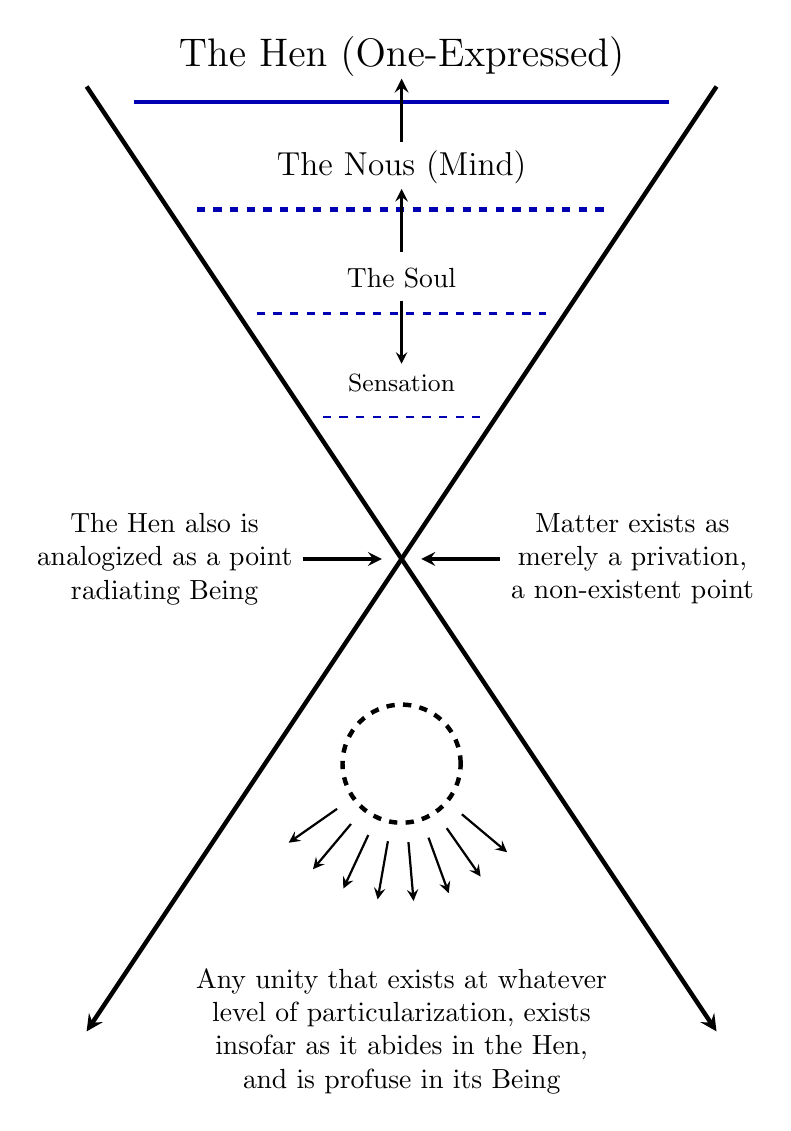
\begin{tikzpicture}	
	\def\w{4}
	\draw[ultra thick,->,>=stealth] (-\w,3*\w)--(\w,0);
	\draw[ultra thick,->,>=stealth] (\w,3*\w)--(-\w,0);
	\node[align=center] at (0,0) {
		Any unity that exists at whatever\\ 
		level of particularization, exists\\ 
		insofar as it abides in the Hen,\\
		and is profuse in its Being
	};
	
	\draw[very thick,<-,>=stealth] (0.25,1.5*\w)--++(1,0) %
	node[align=center,right] {
		Matter exists as \\
		merely a privation, \\
		a non-existent point
	};
	\draw[very thick,<-,>=stealth] (-0.25,1.5*\w)--++(-1,0) %
	node[align=center,left] {
		The Hen also is \\
		analogized as a point \\
		radiating Being
	};
	
	%CIRCLE
	\draw[dashed,ultra thick] (0,0.85*\w) circle (0.75cm);
	\foreach \i in {1,...,8} 
		\draw[thick,->,>=stealth] ({1*cos(200+15*\i)},{0.85*\w+1*sin(200+15*\i)}) -- ({1.75*cos(200+15*\i)},{0.85*\w+1.75*sin(200+15*\i)});
	
	%TOP LINES
	\node[above] at (0,3.0*\w) {\Large The Hen (One-Expressed)};
	\node[above] at (0,2.66*\w) {\large The Nous (Mind)};
	\node[above] at (0,2.33*\w) {The Soul};
	\node[above] at (0,2*\w) {\small Sensation};
	
	\draw[blue!70!black,ultra thick] (-0.85*\w,2.95*\w)--(0.85*\w,2.95*\w); %hen
	\draw[dashed,blue!70!black,ultra thick] (-0.65*\w,2.61*\w)--(0.65*\w,2.61*\w); %nous
	\draw[dashed,blue!70!black,very thick] (-0.46*\w,2.28*\w)--(0.46*\w,2.28*\w); %soul
	\draw[dashed,blue!70!black,thick] (-0.25*\w,1.95*\w)--(0.25*\w,1.95*\w); %sensation
	
	\draw[thick,->,>=stealth] (0,2.32*\w)--++(0,-0.8); %soul--sensation
	\draw[line width=1pt,->,>=stealth] (0,2.475*\w)--++(0,0.8); %soul--nous
	\draw[very thick,->,>=stealth] (0,2.825*\w)--++(0,0.8); %nous--hen
	\end{tikzpicture}
	
\end{document}